% Copyright 2018-2019 Melvin Eloy Irizarry-Gelpí
\setcounter{chapter}{4}
\chapter{Capacitors and Inductors}
%%%%%%%%%%%%%%%%%%%%%%%%%%%%%%%%%%%%%%%%%%%%%%%%%%%%%%%%%%%%%%%%%%%%%%%%%%%%%%%%
In this experiment you will learn about circuits with capacitors and inductors.
%%%%%%%%%%%%%%%%%%%%%%%%%%%%%%%%%%%%%%%%%%%%%%%%%%%%%%%%%%%%%%%%%%%%%%%%%%%%%%%%
\section{Preliminary}
%%%%%%%%%%%%%%%%%%%%%%%%%%%%%%%%%%%%%%%%%%%%%%%%%%%%%%%%%%%%%%%%%%%%%%%%%%%%%%%%
A given component in an electric circuit can have many physical properties. Among them are resistance, capacitance, and inductance.
%%%%%%%%%%%%%%%%%%%%%%%%%%%%%%%%%%%%%%%%%%%%%%%%%%%%%%%%%%%%%%%%%%%%%%%%%%%%%%%%
\subsection{Resistance and Resistors}
%%%%%%%%%%%%%%%%%%%%%%%%%%%%%%%%%%%%%%%%%%%%%%%%%%%%%%%%%%%%%%%%%%%%%%%%%%%%%%%%
By now, electrical \textbf{resistance} should be familiar. The \textbf{SI unit} for electrical resistance is the \textbf{ohm}:
\begin{equation}
	1 \text{ ohm} = 1\;\Omega = 1 \text{ V/A}
\end{equation}
Here, V is volt (voltage) and A is ampere (current). A component in a circuit with a fixed amount of resistance is called a \textbf{resistor}. The mathematical symbol for resistance is $R$.
%%%%%%%%%%%%%%%%%%%%%%%%%%%%%%%%%%%%%%%%%%%%%%%%%%%%%%%%%%%%%%%%%%%%%%%%%%%%%%%%
\subsection{Capacitance and Capacitors}
%%%%%%%%%%%%%%%%%%%%%%%%%%%%%%%%%%%%%%%%%%%%%%%%%%%%%%%%%%%%%%%%%%%%%%%%%%%%%%%%
Another important property is \textbf{capacitance}. The \textbf{SI unit} for capacitance is the \textbf{farad}:
\begin{equation}
	1 \text{ farad} = 1 \text{ F} = 1 \text{ C/V}
\end{equation}
Here, C is coulomb (electric charge) and V is volt (voltage). In some ways, capacitance measures the amount of electric charge needed to sustain an electric potential difference (i.e. a voltage). The mathematical symbol for capacitance is $C$.

A component in a circuit with a fixed amount of capacitance is called a \textbf{capacitor}. You can think of a capacitor as two parallel plates of conducting material where equal but opposite amounts of electric charge can accumulate.
%%%%%%%%%%%%%%%%%%%%%%%%%%%%%%%%%%%%%%%%%%%%%%%%%%%%%%%%%%%%%%%%%%%%%%%%%%%%%%%%
\subsection{Inductance and Inductors}
%%%%%%%%%%%%%%%%%%%%%%%%%%%%%%%%%%%%%%%%%%%%%%%%%%%%%%%%%%%%%%%%%%%%%%%%%%%%%%%%
The last property is \textbf{inductance}, which is like a magnetic cousin of capacitance. The \textbf{SI unit} for inductance is the \textbf{henry}:
\begin{equation}
	1 \text{ henry} = 1 \text{ H} = 1 \text{ T m}^{2}\text{/A}
\end{equation}
Here, T is tesla (magnetic field), m$^{2}$ is square meter (area), and A is ampere (current). In some ways, inductance measures the amount of magnetic flux produced by a current. The mathematical symbol for inductance is $L$.

A component in a circuit with a fixed amount of inductance is called an \textbf{inductor}. You can think of an inductor as a solenoid coil with a given amount of loops, with each loop enclosing some amount of area.
%%%%%%%%%%%%%%%%%%%%%%%%%%%%%%%%%%%%%%%%%%%%%%%%%%%%%%%%%%%%%%%%%%%%%%%%%%%%%%%%
\subsection{Exponential Decay Function}
%%%%%%%%%%%%%%%%%%%%%%%%%%%%%%%%%%%%%%%%%%%%%%%%%%%%%%%%%%%%%%%%%%%%%%%%%%%%%%%%
Before discussing the behavior of current and voltage in circuits with capacitors and inductors, it will be good to review the exponential decay function:
\begin{equation}
    \exp(-t) = e^{-t}
\end{equation}
Here, $e$ is the \textbf{natural base}:
\begin{equation}
    e = 2.71828...
\end{equation}
When $t = 0$, the exponential decay function gives
\begin{equation}
    \exp(0) = 1
\end{equation}
For large values of $t$, the exponential decay function approaches 0:
\begin{equation}
    \exp(-\infty) = 0
\end{equation}
In between $t = 0$ and $t \rightarrow \infty$ you have smaller and smaller values approaching zero.

The exponential decay function is an example of a function that is always positive, and always \textbf{decreasing} towards zero:
\begin{align}
    f(t) = \exp(-t) && 0 < f(t) \leq 1 && 0 \leq t < \infty
\end{align}
Multiplying the exponential decay function by a negative sign produces a function that is always negative, and always \textbf{increasing} towards zero:
\begin{align}
    g(t) = -\exp(-t) && -1 \leq g(t) < 0 && 0 \leq t < \infty
\end{align}
Another important combination is shifting vertically by 1, which gives a function that is always positive, and always \textbf{increasing} towards one:
\begin{align}
    h(t) = 1 - \exp(-t) && 0 \leq h(t) < 1 && 0 \leq t < \infty
\end{align}
Figures \ref{figure.05.f}, \ref{figure.05.g}, and \ref{figure.05.h} provide charts for these three functions.
%%%%%%%%%%%%%%%%%%%%%%%%%%%%%%%%%%%%%%%%%%%%%%%%%%%%%%%%%%%%%%%%%%%%%%%%%%%%%%%%
\subsection{Resistor and Capacitor in Series}
%%%%%%%%%%%%%%%%%%%%%%%%%%%%%%%%%%%%%%%%%%%%%%%%%%%%%%%%%%%%%%%%%%%%%%%%%%%%%%%%
A circuit with a resistor, a capacitor, and a direct-current (DC) source is called an \textbf{RC circuit}. In the simplest RC circuit, the resistor and capacitor are connected in series to the DC source via a particular switch.
%%%%%%%%%%%%%%%%%%%%%%%%%%%%%%%%%%%%%%%%%%%%%%%%%%%%%%%%%%%%%%%%%%%%%%%%%%%%%%%%
\subsubsection{Charging Capacitor}
%%%%%%%%%%%%%%%%%%%%%%%%%%%%%%%%%%%%%%%%%%%%%%%%%%%%%%%%%%%%%%%%%%%%%%%%%%%%%%%%
When the switch is on, and the circuit is complete, the DC source pushes charges out into the circuit in the form of a current. This current causes positive electric charges to accumulate on one of the terminals of the capacitor, and negative electric charges on the other terminal of the capacitor. But the amount of electric charge $Q$ on the capacitor does not increase indefinitely: It settles on a maximum value $Q_{\infty}$. The particular manner in which the amount of \textbf{electric charge} on the capacitor increases with time is an example of an \textbf{exponential} increase:
\begin{equation}
    Q(t) = Q_{\infty} \left[ 1 - \exp\left(-\frac{t}{\tau_{C}}\right) \right]
    \label{eq.05.RC.q.charging}
\end{equation}
Here $Q_{\infty}$ is the amount of charge accumulated on the capacitor after an infinite amount of time, and $t$ correspond to the amount of time after the switch has been opened (the switch is opened at $t = 0$ s). The amount of \textbf{current} corresponds to the rate of change of the electric charge with time:
\begin{equation}
    I(t) = I_{0} \exp\left(-\frac{t}{\tau_{C}}\right)
    \label{eq.05.RC.i.charging}
\end{equation}
For a capacitor with capacitance $C$, the amount of \textbf{voltage} $V_{C}$ across the \textbf{capacitor} is directly proportional to the amount of electric charge accumulated on the capacitor:
\begin{equation}
    V_{C}(t) = \frac{Q(t)}{C} = V_{\infty} \left[ 1 - \exp\left(-\frac{t}{\tau_{C}}\right) \right]
    \label{eq.05.RC.vC.charging}
\end{equation}
The \textbf{voltage} $V_{R}$ across the \textbf{resistor} is directly proportional the the amount of current, via Ohm's law:
\begin{equation}
    V_{R}(t) = R I(t) = V_{\infty} \exp\left(-\frac{t}{\tau_{C}}\right)
    \label{eq.05.RC.vR.charging}
\end{equation}
Here, $V_{\infty}$ is related to $Q_{\infty}$ and/or $I_{0}$ via
\begin{eqnarray}
    V_{\infty} = \frac{Q_{\infty}}{C} = I_{0} R
\end{eqnarray}
The value of $V_{\infty}$ should correspond to the steady voltage across the DC source.

As you can see from (\ref{eq.05.RC.q.charging}), (\ref{eq.05.RC.i.charging}), and (\ref{eq.05.RC.vC.charging}), the amount of charge, current and voltage related to a capacitor all involve exponential functions. The constant $\tau_{C}$ is known as the \textbf{capacitive time constant}. It has units of time (seconds). The value of $\tau_{C}$ sets a time scale for the change in values to occur. The same time scale appears in all three quantities. In an RC circuit, the value of $\tau_{C}$ depends on how much resistance $R$ and capacitance $C$ you have:
\begin{equation}
    \tau_{C} = R C
    \label{eq.05.tauC}
\end{equation}
You can check that, in fact, by multiplying something with ohm units by something with farad units you get something with second units:
\begin{equation}
    1 \text{ ohm} \cdot 1 \text{ F} = \left(1 \text{ V}\cdot\text{ s/C}\right) \cdot \left(1 \text{ C/V}\right) = 1 \text{ s}
\end{equation}
Since the exponential function is a mathematical function that changes very fast, the current will take noise-level values after a time corresponding to about 5 capacitive time constants.
%%%%%%%%%%%%%%%%%%%%%%%%%%%%%%%%%%%%%%%%%%%%%%%%%%%%%%%%%%%%%%%%%%%%%%%%%%%%%%%%
\subsubsection{Discharging Capacitor}
%%%%%%%%%%%%%%%%%%%%%%%%%%%%%%%%%%%%%%%%%%%%%%%%%%%%%%%%%%%%%%%%%%%%%%%%%%%%%%%%
After some time with the switch on, the amount of charge on the capacitor becomes almost constant (close to $Q_{\infty}$), the amount of voltage across the capacitor also becomes almost constant (close to $V_{\infty}$), and the current through the circuit becomes almost zero. Upon opening the circuit by setting the switch off, the DC source stops supporting the charge accumulated on the capacitor, and that amount of charge begins to leave the capacitor. The amount of charge on the capacitor follows a particular manner:
\begin{equation}
    Q(t) = Q_{0} \exp\left(-\frac{t}{\tau_{C}}\right)
    \label{eq.05.RC.q.discharging}
\end{equation}
Here $Q_{0}$ is the amount of charge at the moment that the switch is turned off. The electric current is given by
\begin{equation}
    I(t) = - I_{0} \exp\left(-\frac{t}{\tau_{C}}\right)
    \label{eq.05.RC.i.discharging}
\end{equation}
This behavior is very similar to the behavior of the current (\ref{eq.05.RC.i.charging}) while the capacitor is charging, except that the negative sign indicates the current is in the opposite direction, since the charge is leaving the capacitor. The voltage $V_{C}$ across the \textbf{capacitor} can, again, be found from the amount of electric charge:
\begin{equation}
    V_{C}(t) = \frac{Q(t)}{C} = V_{0} \exp\left(-\frac{t}{\tau_{C}}\right)
    \label{eq.05.RC.vC.discharging}
\end{equation}
The capacitive time constant appears again, and also dictates the time scale for the decrease of the charge, current and voltage across the capacitor during the discharging event. The voltage $V_{R}$ across the \textbf{resistor} can, again, be found from the amount of electric current:
\begin{equation}
    V_{R}(t) = R I(t) = - V_{0} \exp\left(-\frac{t}{\tau_{C}}\right)
\end{equation}
Just as before, there is a relation between $Q_{0}$, $I_{0}$, and $V_{0}$:
\begin{equation}
    V_{0} = \frac{Q_{0}}{C} = I_{0} R
\end{equation}
The value of $V_{0}$ should correspond to the voltage across the capacitor just before the switch is opened.
%%%%%%%%%%%%%%%%%%%%%%%%%%%%%%%%%%%%%%%%%%%%%%%%%%%%%%%%%%%%%%%%%%%%%%%%%%%%%%%%
\subsection{Resistor and Inductor in Series}
%%%%%%%%%%%%%%%%%%%%%%%%%%%%%%%%%%%%%%%%%%%%%%%%%%%%%%%%%%%%%%%%%%%%%%%%%%%%%%%%
A circuit with a resistor, an inductor, and a DC source is called an \textbf{RL circuit}. In the simplest RL circuit, the resistor and inductor are connected in series to the DC source via a particular switch.
%%%%%%%%%%%%%%%%%%%%%%%%%%%%%%%%%%%%%%%%%%%%%%%%%%%%%%%%%%%%%%%%%%%%%%%%%%%%%%%%
\subsubsection{Closed Switch: Rise of Current}
%%%%%%%%%%%%%%%%%%%%%%%%%%%%%%%%%%%%%%%%%%%%%%%%%%%%%%%%%%%%%%%%%%%%%%%%%%%%%%%%
Although an inductor does not accumulate electric charge like a capacitor, the behavior of electric current and voltage across an inductor in an RL circuit also involves exponential functions.

Whereas in an RC circuit the current becomes zero for large time values after closing the switch, in an RL circuit the current rises to a steady value:
\begin{equation}
    I(t) = I_{\infty} \left[ 1 - \exp\left(- \frac{t}{\tau_{L}}\right) \right]
    \label{eq.05.RL.i.rise}
\end{equation}
The \textbf{voltage} $V_{R}$ across the \textbf{resistor} is given by Ohm's law:
\begin{equation}
    V_{R}(t) = R I(t) = V_{\infty} \left[ 1 - \exp\left(- \frac{t}{\tau_{L}}\right) \right]
    \label{eq.05.RL.vR.rise}
\end{equation}
The \textbf{voltage} $V_{L}$ across the \textbf{inductor} is given by
\begin{equation}
    V_{L}(t) = V_{\infty} - V_{R}(t) = V_{\infty} \exp\left(- \frac{t}{\tau_{L}}\right)
    \label{eq.05.RL.vL.rise}
\end{equation}
Here $I_{\infty}$ and $V_{\infty}$ are related via
\begin{equation}
    V_{\infty} = I_{\infty} R
\end{equation}
Instead of $\tau_{C}$, you now have $\tau_{L}$ which corresponds to the \textbf{inductive time constant}. Just like $\tau_{C}$, the value of $\tau_{L}$ depends on the amount of resistance and inductance you have in the circuit:
\begin{equation}
    \tau_{L} = \frac{L}{R}
    \label{eq.05.tauL}
\end{equation}
You can check that in fact, by dividing something with henry units by something with ohm units you get something with second units. 
%%%%%%%%%%%%%%%%%%%%%%%%%%%%%%%%%%%%%%%%%%%%%%%%%%%%%%%%%%%%%%%%%%%%%%%%%%%%%%%%
\subsubsection{Opened Switch: Decay of Current}
%%%%%%%%%%%%%%%%%%%%%%%%%%%%%%%%%%%%%%%%%%%%%%%%%%%%%%%%%%%%%%%%%%%%%%%%%%%%%%%%
After a long time with the switch closed in an RL circuit, the current reaches a steady value. If you now open the switch, the current around the circuit will decay and eventually will become zero:
\begin{equation}
    I(t) = I_{0} \exp\left(- \frac{t}{\tau_{L}}\right)
    \label{eq.05.RL.i.decay}
\end{equation}
Note that unlike for the discharging of the capacitor, where the current actually switches sign, the current here does not switch sign. The voltage $V_{R}$ across the resistor is given by:
\begin{equation}
    V_{R}(t) = R I(t) = V_{0} \exp\left(- \frac{t}{\tau_{L}}\right)
    \label{eq.05.RL.vR.decay}
\end{equation}
The voltage $V_{L}$ across the inductor is given by:
\begin{equation}
    V_{L}(t) = -V_{R}(t) = -V_{0} \exp\left(- \frac{t}{\tau_{L}}\right)
    \label{eq.05.RL.vL.decay}
\end{equation}
All three quantities eventually become zero for large values of time after the switch is opened.
%%%%%%%%%%%%%%%%%%%%%%%%%%%%%%%%%%%%%%%%%%%%%%%%%%%%%%%%%%%%%%%%%%%%%%%%%%%%%%%%
\section{Experiment}
%%%%%%%%%%%%%%%%%%%%%%%%%%%%%%%%%%%%%%%%%%%%%%%%%%%%%%%%%%%%%%%%%%%%%%%%%%%%%%%%
You did experiments for both RC and RL circuits.
%%%%%%%%%%%%%%%%%%%%%%%%%%%%%%%%%%%%%%%%%%%%%%%%%%%%%%%%%%%%%%%%%%%%%%%%%%%%%%%%
\subsection{RC Circuits}
%%%%%%%%%%%%%%%%%%%%%%%%%%%%%%%%%%%%%%%%%%%%%%%%%%%%%%%%%%%%%%%%%%%%%%%%%%%%%%%%
For RC circuits there are two kinds of events: the charging event and the discharging event. In each experiment you measured the voltage across the resistor, the current flowing between the resistor and the capacitor, and the voltage across the capacitor.

For the \textbf{charging event}, the data collection was started with the switch off (i.e. incomplete circuit) and shortly after turned on. You should analyze the \textbf{current} and the \textbf{voltage across the resistor} for such events.

For the \textbf{discharging event}, the data collection was started with the switch on (i.e. complete circuit) and shortly after turned off. You should analyze the \textbf{voltage across the capacitor} for such events.

There are nine runs of data:
\begin{itemize}
    \item Run 1: Charging capacitor with $R = 10$ ohm and $C = 2.5 \times 10^{-2}$ F.
	\item Run 2: Discharging capacitor with $R = 10$ ohm and $C = 2.5 \times 10^{-2}$ F.
	\item Run 3: Charging capacitor with $R = 51$ ohm and $C = 2.5 \times 10^{-2}$ F.
	\item Run 4: Discharging capacitor with $R = 51$ ohm and $C = 2.5 \times 10^{-2}$ F.
	\item Run 5: Charging capacitor with $R = 68$ ohm and $C = 2.5 \times 10^{-2}$ F.
	\item Run 6: Discharging capacitor with $R = 68$ ohm and $C = 2.5 \times 10^{-2}$ F.
	\item Run 7: Discharging capacitor with $R = 2.2 \times 10^{4}$ ohm and $C = 10^{-5}$ F.
	\item Run 8: Discharging capacitor with $R = 4.7 \times 10^{4}$ ohm and $C = 10^{-5}$ F.
	\item Run 9: Discharging capacitor with $R = 10^{5}$ ohm and $C = 10^{-5}$ F.
\end{itemize}
Each time the resistance or the capacitance changes, the time constant $\tau_{C}$ will also change.
%%%%%%%%%%%%%%%%%%%%%%%%%%%%%%%%%%%%%%%%%%%%%%%%%%%%%%%%%%%%%%%%%%%%%%%%%%%%%%%%
\subsection{RL Circuits}
%%%%%%%%%%%%%%%%%%%%%%%%%%%%%%%%%%%%%%%%%%%%%%%%%%%%%%%%%%%%%%%%%%%%%%%%%%%%%%%%
For RL circuits there are also two kinds of events: the rising current with a closed switch, and the decaying current with an opened switch. Just like for the RC circuit, for each RL circuit experiment you measure the voltage across the resistor, the current flowing between the resistor and the inductor, and the voltage across the inductor. Because the inductive time constants are so small, the data acquisition needs to be activated with the triggering feature.

There are eight runs of data:
\begin{itemize}
    \item Run 1: $R = 10$ ohm, one inductor without metallic core ($L = 0.005$ H expected).
    \item Run 2: $R = 10$ ohm, one inductor with metallic core (unknown $L$ expected).
    \item Run 3: $R = 5$ ohm, one inductor without metallic core ($L = 0.005$ H expected).
    \item Run 4: $R = 5$ ohm, one inductor with metallic core (unknown $L$ expected).
    \item Run 5: $R = 10$ ohm, two inductors without metallic core ($L = 0.01$ H expected).
    \item Run 6: $R = 10$ ohm, two inductors with metallic core (unknown $L$ expected).
    \item Run 7: $R = 5$ ohm, two inductors without metallic core ($L = 0.01$ H expected).
    \item Run 8: $R = 5$ ohm, two inductors with metallic core (unknown $L$ expected).
\end{itemize}
Each time the resistance or the inductance changes, the time constant $\tau_{L}$ will also change.
%%%%%%%%%%%%%%%%%%%%%%%%%%%%%%%%%%%%%%%%%%%%%%%%%%%%%%%%%%%%%%%%%%%%%%%%%%%%%%%%
\section{Analysis}
%%%%%%%%%%%%%%%%%%%%%%%%%%%%%%%%%%%%%%%%%%%%%%%%%%%%%%%%%%%%%%%%%%%%%%%%%%%%%%%%
The common feature of $f(t)$, $g(t)$, and $h(t)$ above is that they all settle on steady values for infinite time after $t = 0$. In an experiment, you do not have an infinite amount of time, so a relevant question is how long corresponds to infinite time. Since you are using imperfect sensors to measure current and voltage, after some time of decreasing towards zero 
%%%%%%%%%%%%%%%%%%%%%%%%%%%%%%%%%%%%%%%%%%%%%%%%%%%%%%%%%%%%%%%%%%%%%%%%%%%%%%%%
\section{My Data}
%%%%%%%%%%%%%%%%%%%%%%%%%%%%%%%%%%%%%%%%%%%%%%%%%%%%%%%%%%%%%%%%%%%%%%%%%%%%%%%%
...
%%%%%%%%%%%%%%%%%%%%%%%%%%%%%%%%%%%%%%%%%%%%%%%%%%%%%%%%%%%%%%%%%%%%%%%%%%%%%%%%
\section{Your Data}
%%%%%%%%%%%%%%%%%%%%%%%%%%%%%%%%%%%%%%%%%%%%%%%%%%%%%%%%%%%%%%%%%%%%%%%%%%%%%%%%
...
%%%%%%%%%%%%%%%%%%%%%%%%%%%%%%%%%%%%%%%%%%%%%%%%%%%%%%%%%%%%%%%%%%%%%%%%%%%%%%%%
\newpage
\section{Your Lab Report}
%%%%%%%%%%%%%%%%%%%%%%%%%%%%%%%%%%%%%%%%%%%%%%%%%%%%%%%%%%%%%%%%%%%%%%%%%%%%%%%%
...
%%%%%%%%%%%%%%%%%%%%%%%%%%%%%%%%%%%%%%%%%%%%%%%%%%%%%%%%%%%%%%%%%%%%%%%%%%%%%%%%
\newpage
\section{Tables}
%%%%%%%%%%%%%%%%%%%%%%%%%%%%%%%%%%%%%%%%%%%%%%%%%%%%%%%%%%%%%%%%%%%%%%%%%%%%%%%%
...
%%%%%%%%%%%%%%%%%%%%%%%%%%%%%%%%%%%%%%%%%%%%%%%%%%%%%%%%%%%%%%%%%%%%%%%%%%%%%%%%
\newpage
\section{Figures}
%%%%%%%%%%%%%%%%%%%%%%%%%%%%%%%%%%%%%%%%%%%%%%%%%%%%%%%%%%%%%%%%%%%%%%%%%%%%%%%%
\begin{figure}[ht]
    \centering
    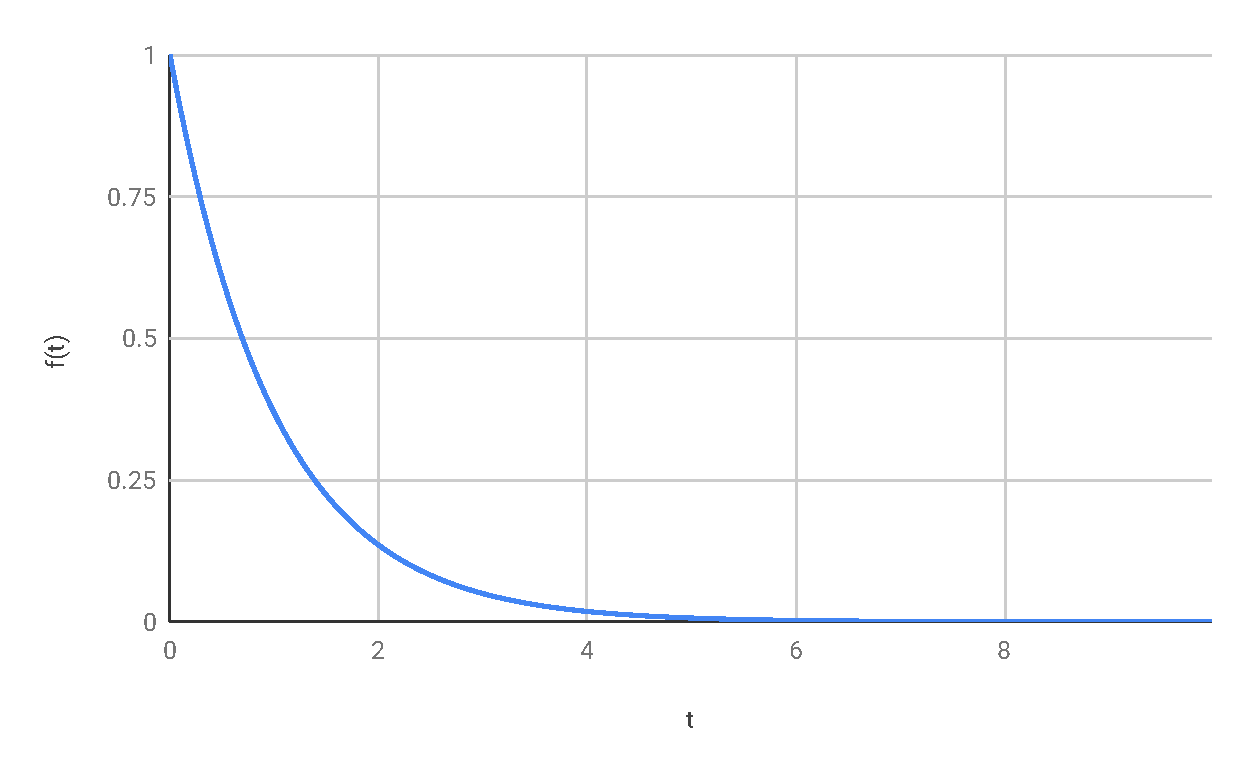
\includegraphics[scale=0.74]{image/05-RC-RL/f.pdf}
    \caption{Function $f(t)$}
    \label{figure.05.f}
\end{figure}
%%%%%%%%%%%%%%%%%%%%%%%%%%%%%%%%%%%%%%%%%%%%%%%%%%%%%%%%%%%%%%%%%%%%%%%%%%%%%%%%
\begin{figure}[ht]
    \centering
    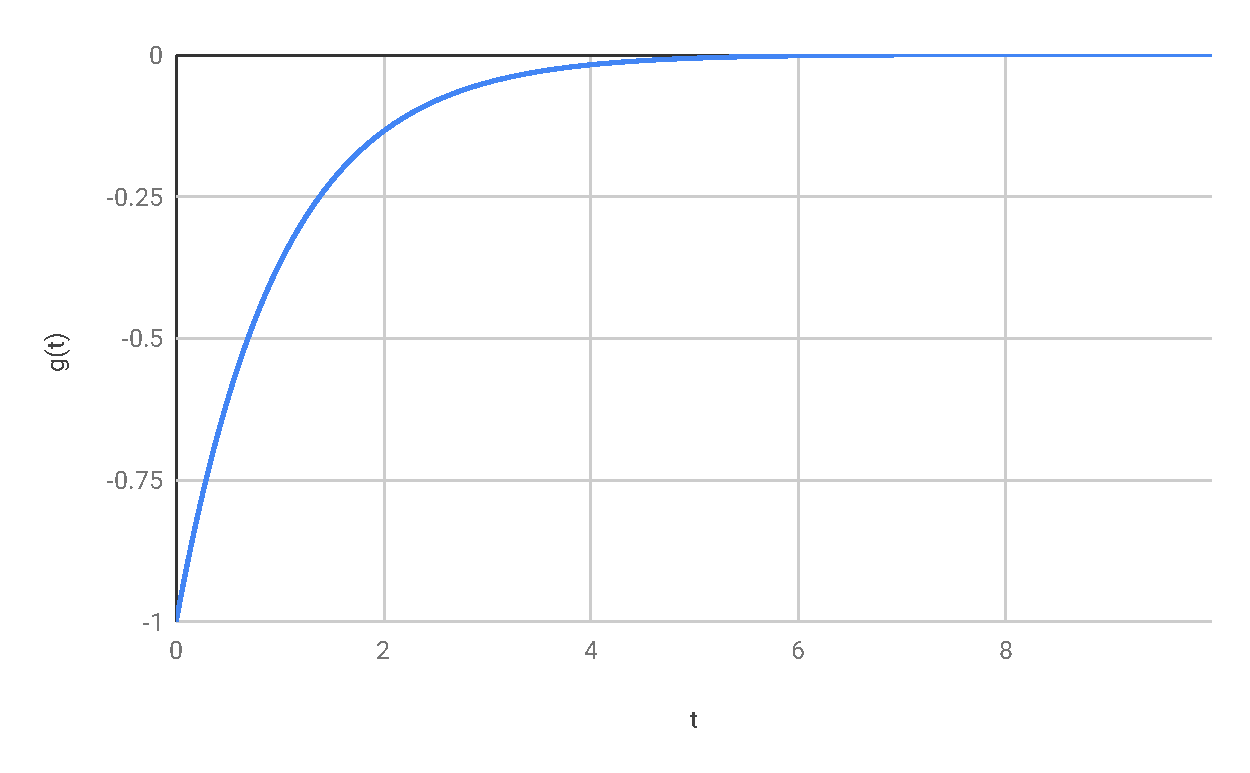
\includegraphics[scale=0.74]{image/05-RC-RL/g.pdf}
    \caption{Function $g(t)$}
    \label{figure.05.g}
\end{figure}
%%%%%%%%%%%%%%%%%%%%%%%%%%%%%%%%%%%%%%%%%%%%%%%%%%%%%%%%%%%%%%%%%%%%%%%%%%%%%%%%
\begin{figure}[ht]
    \centering
    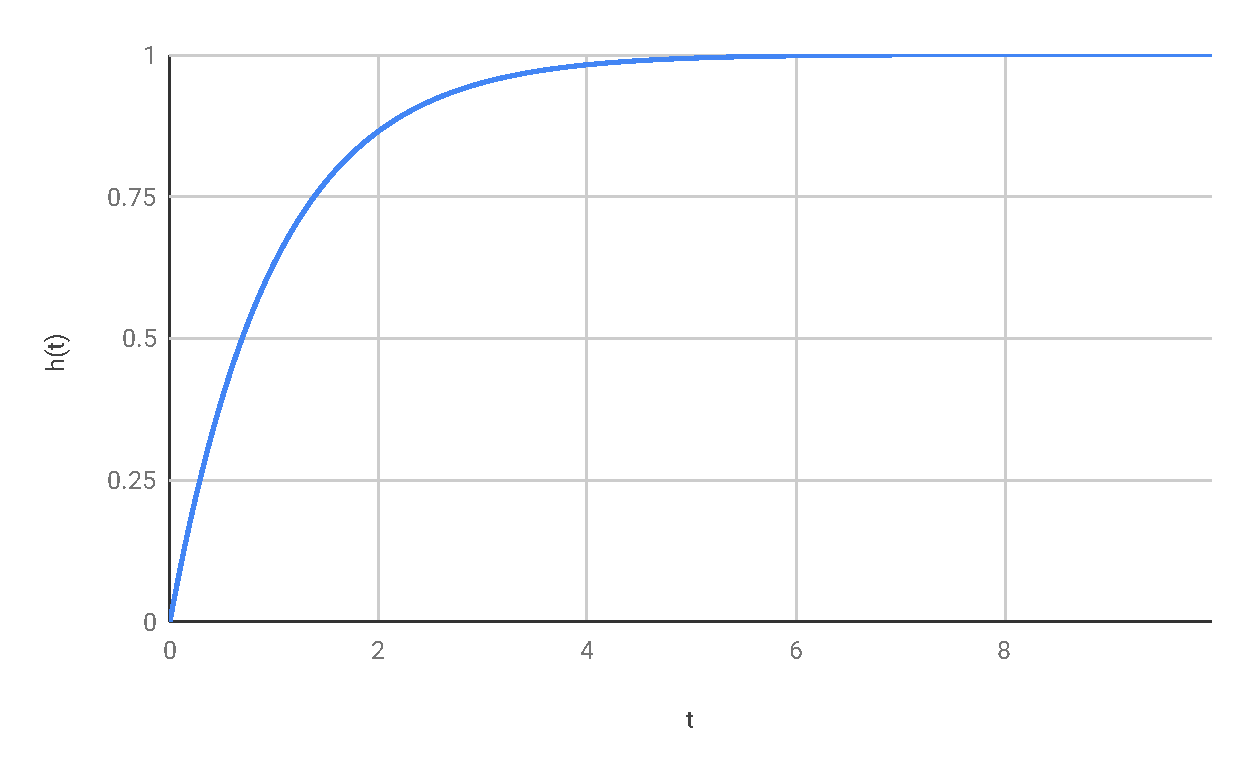
\includegraphics[scale=0.74]{image/05-RC-RL/h.pdf}
    \caption{Function $h(t)$}
    \label{figure.05.h}
\end{figure}